\pdfoutput=1
\documentclass[aps,prd, amsmath,amssymb,superscriptaddress,showkeys,nofootinbib,reprint,preprintnumbers]{revtex4-1}
\usepackage{color}
\usepackage{aas_macros}
\usepackage{hyperref,breakurl}
\usepackage[usenames,dvipsnames]{xcolor}
\usepackage{dcolumn}
\usepackage{bm}
\usepackage{hyperref}
\usepackage{array}
\usepackage{dcolumn}

\usepackage{amsmath,amssymb,latexsym,times}
\DeclareMathOperator\arctanh{arctanh}

\usepackage{todonotes}
\newcommand{\verify}[1]{\textcolor{red}{\textbf{{#1}}}}

\newcommand\assign[1]{\todo[color=RoyalPurple!40, inline, size=\small]{Contributing: #1}}
\newcommand\troxel[1]{\todo[color=cyan!40, inline, size=\small]{Troxel: #1}}
 
\newcommand\green[1]{\textcolor{green}{#1}}

\begin{document}

\title{A synthetic WFIRST survey: Simulation suite and the impact of wavefront errors on weak lensing}

%\author{Troxel, M.A.}
%\email{michael.troxel@duke.edu}
\author{and others}

\collaboration{WFIRST HLS Cosmology SIT}

\noaffiliation

\date{\today}

\label{firstpage}

\begin{abstract}
\end{abstract}

\keywords{}

\maketitle

%\tableofcontents

\section{Introduction}\label{sec:intro}

\begin{itemize}
\item DE/cosmology context
\item motivation for WFIRST in context of other stage iii and stage iv surveys
\item cosmology sit
\item goals of paper
\end{itemize}


The nature of dark energy, which drives cosmic acceleration in the Universe, remains one of the most fundamental mysteries in physics twenty years after its discovery \cite{}. 
A number of new experiments have been undertaken to probe dark energy using a variety of physical phenomena, including baryon acoustic oscillations, numbers and masses of galaxy clusters, galaxy clustering, redshift space distortions, Type Ia supernovae, and weak gravitational lensing. 
Current generation experiments are limited to some subset of these probes, but have already begun to expose interesting questions about the soundness of our standard cosmological model, Lambda-Cold Dark Matter (LCDM) that will require more and better data to resolve. 
The Wide-Field InfraRed Space Telescope (WFIRST) has been designed to take advantage of all of these probes to study dark energy with unprecedented systematic control \cite{}.

In the past few years, the current generation of ground-based weak lensing experiments like the Dark Energy Survey (DES), Hyper-Suprime Cam (HSC), and Kilo-Degree Survey (KiDS) have reached levels of precision that rival the previously best possible cosmological constraints including dark energy \cite{}. 
These surveys have spurred the development of revolutionary algorithms and methods for galaxy shape measurement and weak lensing analysis \cite{}, highlighting the immense power of weak lensing to unravel the fundamental mysteries we face in cosmology today. 

By the planned launch of WFIRST in 2025, we will have final results from the ongoing generation of weak lensing experiments (DES, HSC, and KiDS) and preliminary results from the Dark Energy Spectroscopic Instrument (DESI), the Large Synoptic Survey Telescope (LSST), and the Euclid mission. 
Faced with the unknown discovery potential of these experiments in the early 2020s, it is vital to maintain the agility and flexibility of the WFIRST mission to respond with the best possible science, particularly in what is likely to be a systematics dominated weak lensing field.
The process of quantifying empirically the robustness of the design requirements of the WFIRST mission for weak lensing now in Phase B of the mission development is a critical task that this paper will attempt to address. 
Precise control of these systematics at the statistical precision offered by current WFIRST mission forecasts will enable WFIRST to play the likely role of arbiter in the study of new discoveries made in the early years of LSST and Euclid.

We present in this paper a set of synthetic WFIRST imaging surveys covering approx. 6 sq. deg. in one filter: a fiducial set of images and 11 variations in ways the PSF could be mis-estimated. 
It incorporates realistic distributions of photometric properties for galaxies and stars; complex analytic galaxy models; a simulated fiducial five year, 2000 sq. deg. observation strategy for the survey; and realistic detector effects, PSF models, and WCS solutions that match current (Cycle 7) design specifications. 
We use a blending-free version of this simulation to test the impact on weak lensing science of a variety of PSF or wave-front errors, including static, low-, and high-frequency biases. 

(insert standard toc para) 


\section{WFIRST and requirements}\label{sec:wfirst}

\begin{itemize}
\item What WFIRST is \& timeline
\item Previous requirements information
\item context in broader sit work
\item transition to empirical validation (next section)
\end{itemize}

\def\arraystretch{1.4}
\setlength{\tabcolsep}{4pt}
\begin{table}
\caption{Table}
\label{table:values}
\begin{center}
\begin{tabular}{lcccc }
\hline
\hline
%Parameter & $o$CDM & $w$CDM & $w$CDM (Ext) & Flat Prior \\ 
%\hline
%$\Omega_m$                                                  & $0.299^{+0.024}_{-0.020}$  &  $0.300^{+0.023}_{-0.021}$  & $0.303^{+0.007}_{-0.009}$ & [0.1, 0.9] \\
%$\Omega_b$                                                   & $0.069^{+0.009}_{-0.012}$   & $0.064^{+0.013}_{-0.009}$  & $0.048^{+0.001}_{-0.001}$ & [0.03, 0.12] \\
%$\Omega_k$                                                   & $0.252^{+0.095}_{-0.14}$     & 0 & 0 & [-0.1, 0.5] \\
%$\Omega_\Lambda$                                       & $0.47^{+0.14}_{-0.12}$        & $0.700^{+0.021}_{-0.023}$  & $0.697^{+0.009}_{-0.007}$ & Derived \\
%$w$                                                                 & $-1$                                      & $-0.80^{+0.09}_{-0.11}$       & $-1.02^{+0.03}_{-0.04}$ & [-2, -0.33] \\
%$S_8$  							    & $0.801^{+0.028}_{-0.026}$  & $0.786^{+0.029}_{-0.019}$   & $0.814^{+0.016}_{-0.011}$ & Derived \\ 
\hline
\hline
\end{tabular}
\end{center}
\end{table}

\begin{figure*}
\begin{center}
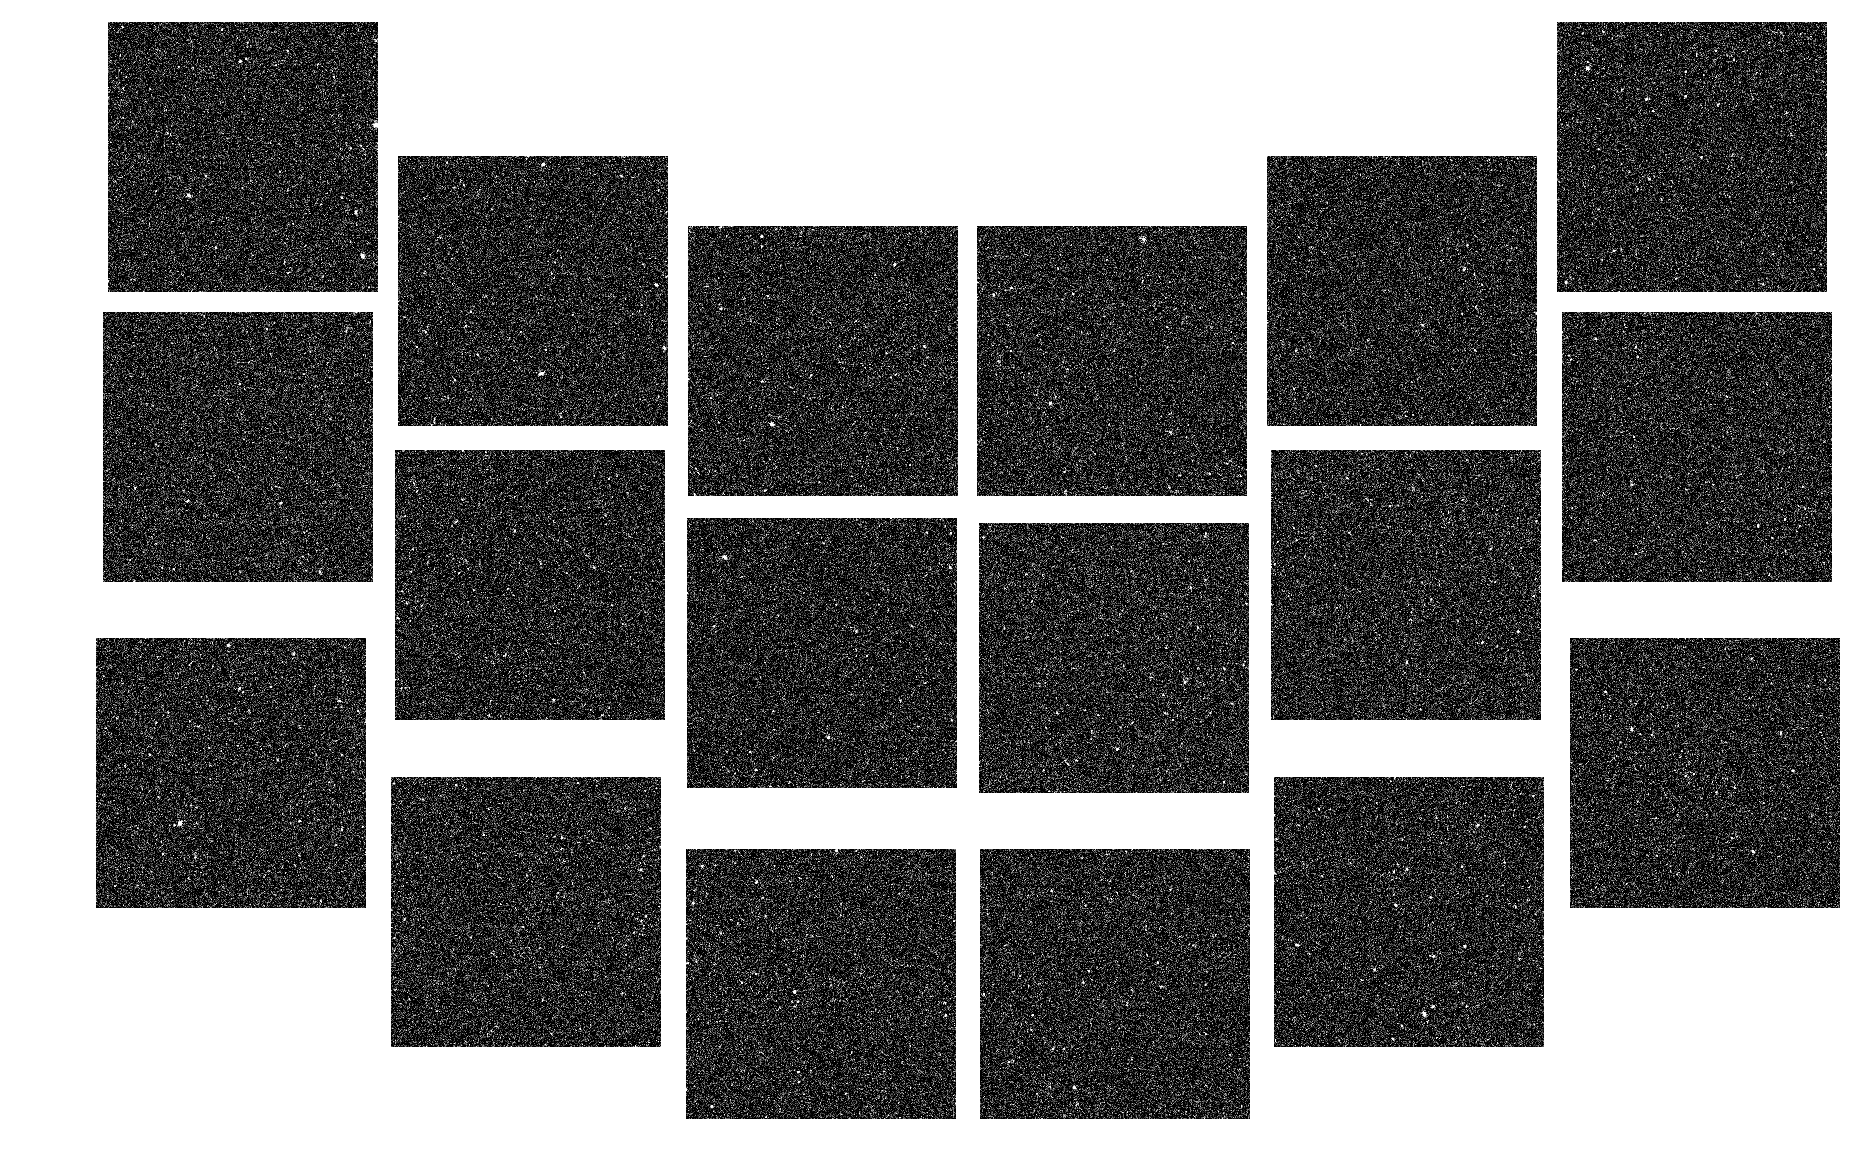
\includegraphics[width=\textwidth]{figures/fov.pdf}
\end{center}
\caption[]{
A simulated field-of-view (FOV) from the fiducial simulation matching Cycle 7 specifications. The WFIRST FOV is 0.282 deg$^2$, composed of 18 near-IR Sensor Chip Arrays (H4RGs). This FOV is 200 times the area of the Hubble Space Telescope Wide Field Camera 3 FOV and 90 times that of its Advanced Camera for Surveys. (check chip orientation)
\label{fig:fov}}
\end{figure*}

\begin{figure}
\begin{center}
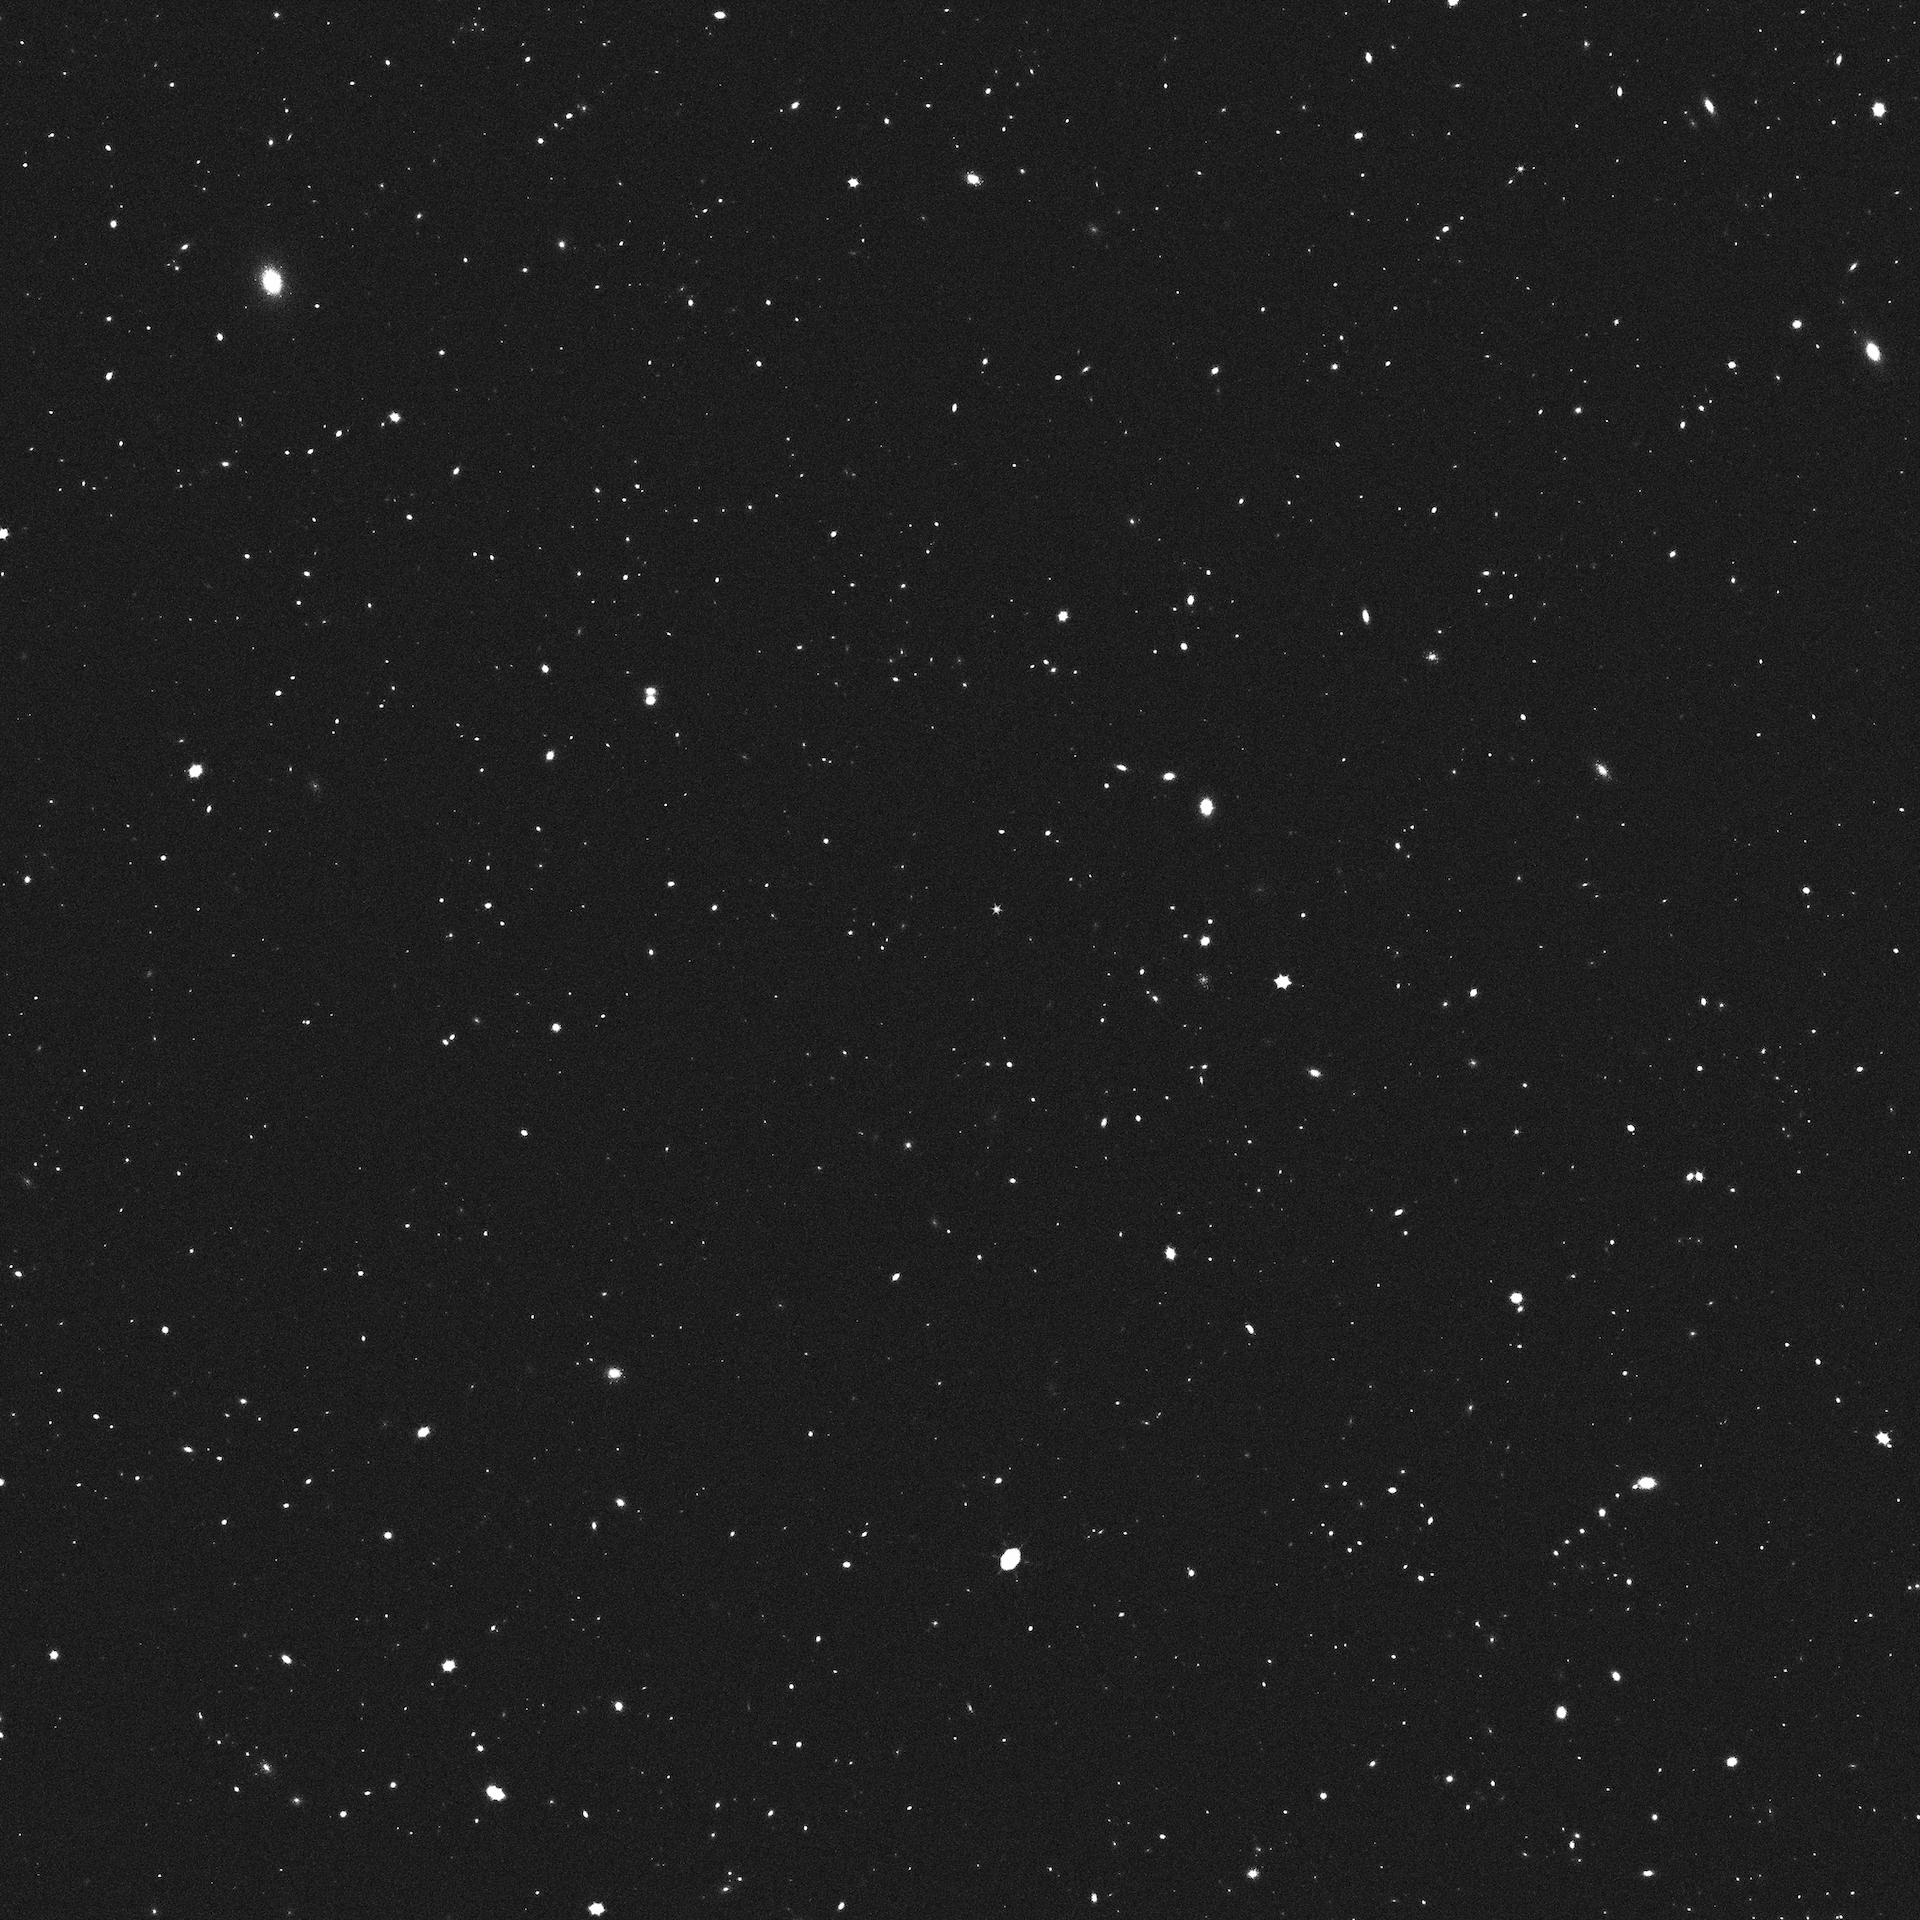
\includegraphics[width=\columnwidth]{figures/sca1.png}
\end{center}
\caption[]{
A simulated WFIRST Sensor Chip Array (SCA). Each SCA (HgCdTe H4RG) has a useable pixel grid of 4088$\times$4088, with a pixel scale of 0.11''. One interesting feature can be seen in the relatively bright galaxy in the lower middle part of the SCA, for which six faint diffraction spikes due to the WFIRST secondary mirror support struts are visible.
\label{fig:sca}}
\end{figure}

\begin{figure}
\begin{center}
\includegraphics[width=\columnwidth]{figures/galaxies.pdf}
\end{center}
\caption[]{
Galaxies, avg. 40 per sq arcmin, dist. from buzzard, phot/morph props from candels catalog
\label{fig:galaxies}}
\end{figure}

\begin{figure}
\begin{center}
\includegraphics[width=\columnwidth]{figures/stars.pdf}
\end{center}
\caption[]{
Stars, avg. 2.5 per sq. arcmin, from galaxia
\label{fig:stars}}
\end{figure}

\begin{figure*}
\begin{center}
\includegraphics[width=\textwidth]{figures/hist.pdf}
\end{center}
\caption[]{
True galaxy and star properties.
\label{fig:hist}}
\end{figure*}

\begin{figure}
\begin{center}
\includegraphics[width=\columnwidth]{figures/pointings.pdf}
\end{center}
\caption[]{
Pointings that overlap the simulated region (non-shaded). The color of each marker shows the position angle of the focal plane.
\label{fig:pointings}}
\end{figure}

\begin{figure*}
\begin{center}
\includegraphics[width=\textwidth]{figures/dates.pdf}
\end{center}
\caption[]{
Dates of observations (is this useful? hard to make it readable)
\label{fig:dates}}
\end{figure*}

\begin{figure}
\begin{center}
\includegraphics[width=\columnwidth]{figures/psf.pdf}
\end{center}
\caption[]{
Example oversampled PSF model compared to native pixel PSF, SCA 1. Top row - full resolution, bottom row - approx. used in sim, left - native pixel scale, right - oversample factor 8
\label{fig:pointings}}
\end{figure}


\section{Simulation suite}\label{sec:sim}

\begin{itemize}
\item We have developed a realistic synthetic survey 
\item into to a synthetic survey and necessary components
\item galsim framework and cycle 7 (\verify{6?}) baseline
\item Detailed description of simulation suite components
\end{itemize}

To empirically test weak lensing requirements, methods, and algorithms in WFIRST, we have designed a sufficiently complex synthetic survey that, while not entirely realistic in all object properties, contains sufficiently complex objects as to enable informative tests and preliminary algorithm development. This synthetic survey utilizes several external simulation and data sources, which are described in the following subsections, and generates WFIRST-like imaging using the GalSim framework and its WFIRST module. The simulation framework is generally capable of producing a full WFIRST HLS imaging survey in all filters matching Cycle 7 specifications. Figure \ref{fig:fov} shows an example pointing produced in the fiducial simulation, and Fig. \ref{fig:sca} shows a larger view of one of the SCAs. Performance details are provided in Appendix \cite{app:performance}. 

\subsection{GalSim}



\subsubsection{Implemented detector effects}


\subsection{Galaxy catalog}

The input galaxy catalog is created using a simulated galaxy distribution on the sky taken from one realization of the Buzzard simulation \cite{1901.02401,wechsler 2019}, to introduce realistic galaxy clustering. Each galaxy is then assigned a random set of photometric properties matching a galaxy from a sample based on the Candels survey that simulates the fiducial WFIRST weak lensing sample selection \cite{}. We show the galaxy distribution in Fig. \ref{fig:galaxies}. We use a galaxy density that is approx. 40 arcmin$^{-2}$. In Fig. \ref{fig:hist}, we show the distributions of size, redshift, and H158 magnitude in the Candels sample. We discard less than 1\% of the largest objects in the shape measurement stage, however, due to a maximum postage stamp size restriction. In general, the input distribution and properties of galaxies can be easily modified by configuration (i.e., specifying a different input galaxy catalog).

\verify{Need lensing selection cuts and maybe short description of candels sample.}

\subsection{Star catalog}

We simulate the positions and magnitudes in WFIRST bandpasses of input stars using the galaxy simulation Galaxia \cite{}. 

\subsection{Survey strategy}
\subsection{Current implementation}



\section{Impact of wavefront errors}\label{sec:results}

\begin{itemize}
\item background on psf and wavefront errors
\item details of wfirst psf in cycle 7 (\verify{6?}) baseline
\item summary of approach 
\end{itemize}

In this paper, we focus on empirical tests of weak lensing requirements for wave front model control (i.e., the PSF) in WFIRST.

\subsection{Static biases}\label{sec:static}

Describe static bias cases

\subsection{High-frequency biases}\label{sec:low}

Describe high-frequency bias cases

\subsection{Low-frequency biases}\label{sec:high}

Describe low-frequency bias cases

\subsection{results}\label{sec:results}

present results in some way

\section{Conclusion}\label{sec:conclusion}

wrap-up

future work and timeline

\section*{Acknowledgements}

This work used resources on the CCAPP condo of the Ruby Cluster at the Ohio Supercomputing Center \cite{OhioSupercomputerCenter1987} and ...OSG, Duke.... Plots in this manuscript were produced partly with \textsc{Matplotlib} \cite{Hunter:2007}, and it has been prepared using NASA's Astrophysics Data System Bibliographic Services.

\bibliographystyle{apsrev4-1}
\bibliography{wfirst_imsim_paper1}

\label{lastpage}

\end{document}
